\subsection{Cas d'utilisation separes par acteur}

Les diagrammes suivants sont produits avec PlantUML. Chaque acteur dispose d'un diagramme separe afin de rendre les responsabilites plus lisibles et d'eviter un diagramme global trop charge.

\subsubsection{Visiteur}

\begin{figure}[H]
  \centering
  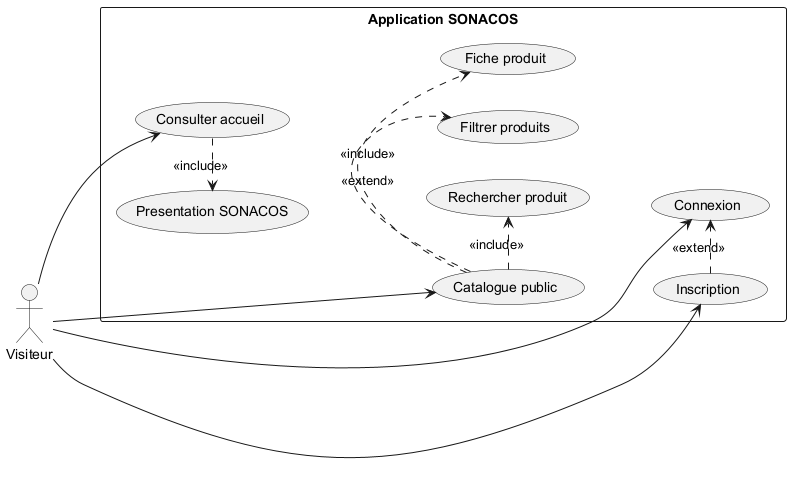
\includegraphics[width=0.92\textwidth,height=0.62\textheight,keepaspectratio]{usecase_visiteur.png}
  \caption{Diagramme PlantUML des cas d'utilisation du visiteur}
  \label{fig:uc-plantuml-visiteur}
\end{figure}

\paragraph{Objectif.}
Le visiteur utilise l'application sans authentification pour decouvrir l'offre SONACOS, consulter les produits disponibles et acceder aux pages d'inscription ou de connexion.

\paragraph{Scenario nominal.}
\begin{enumerate}
  \item Le visiteur ouvre la page d'accueil de l'application.
  \item Le systeme affiche une présentation claire de SONACOS, les grandes familles de produits et les acces principaux.
  \item Le visiteur ouvre le catalogue public.
  \item Le systeme affiche les produits actifs avec image, famille, reference, disponibilite, prix en MAD, conditionnement, stock et livraison.
  \item Le visiteur recherche un produit par nom ou reference.
  \item Le systeme conserve les criteres et affiche les resultats correspondants.
  \item Le visiteur clique sur une carte produit.
  \item Le systeme ouvre la fiche produit complète dans une page dediee.
\end{enumerate}

\paragraph{Cas alternatifs.}
\begin{itemize}
  \item Si aucun produit ne correspond à la recherche, le systeme affiche un etat vide clair.
  \item Si le visiteur veut commander, le systeme l'oriente vers la connexion ou l'inscription.
  \item Si un produit n'est plus actif, il n'apparait plus dans le catalogue public.
\end{itemize}

\subsubsection{Client}

\begin{figure}[H]
  \centering
  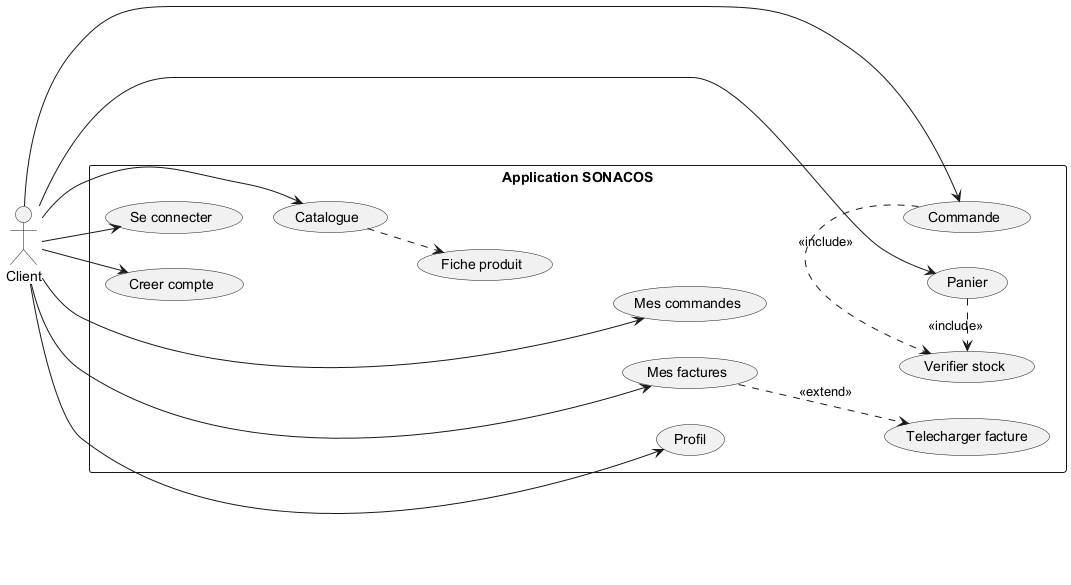
\includegraphics[width=0.92\textwidth,height=0.62\textheight,keepaspectratio]{usecase_client.png}
  \caption{Diagramme PlantUML des cas d'utilisation du client}
  \label{fig:uc-plantuml-client}
\end{figure}

\paragraph{Objectif.}
Le client prepare ses achats depuis le catalogue, gere son panier, passe commande, suit l'avancement et telecharge ses factures lorsque celles-ci sont disponibles.

\paragraph{Preconditions.}
\begin{itemize}
  \item Le client possede un compte actif ou cree un compte depuis la page d'inscription.
  \item Les produits commandes doivent etre actifs et disposer d'un stock suffisant.
  \item Les factures sont telechargeables uniquement apres generation par le systeme.
\end{itemize}

\paragraph{Scenario nominal.}
\begin{enumerate}
  \item Le client se connecte avec son adresse e-mail et son mot de passe.
  \item Le back-end verifie les identifiants et retourne un jeton JWT.
  \item Le front-end redirige le client vers son espace personnel.
  \item Le client consulte le catalogue et ouvre une fiche produit.
  \item Il ajoute un produit au panier en choisissant une quantite.
  \item Le systeme calcule le sous-total de la ligne et le total du panier.
  \item Le client modifie si besoin la quantite ou supprime un article.
  \item Le client confirme la commande.
  \item Le systeme contrôle le stock, cree la commande et enregistre les lignes commandees.
  \item Le client consulte la commande dans son historique.
  \item Lorsque la facture existe, le client la telecharge depuis son espace factures.
\end{enumerate}

\paragraph{Cas alternatifs.}
\begin{itemize}
  \item Si le mot de passe est incorrect, le systeme affiche un message d'erreur sans connecter l'utilisateur.
  \item Si le stock est insuffisant, la commande n'est pas validee et le client est informe.
  \item Si la facture n'est pas encore disponible, le bouton de telechargement reste indisponible ou affiche un message explicite.
  \item Si le compte est desactive par l'administrateur, la connexion est refusee.
\end{itemize}

\subsubsection{Gestionnaire}

\begin{figure}[H]
  \centering
  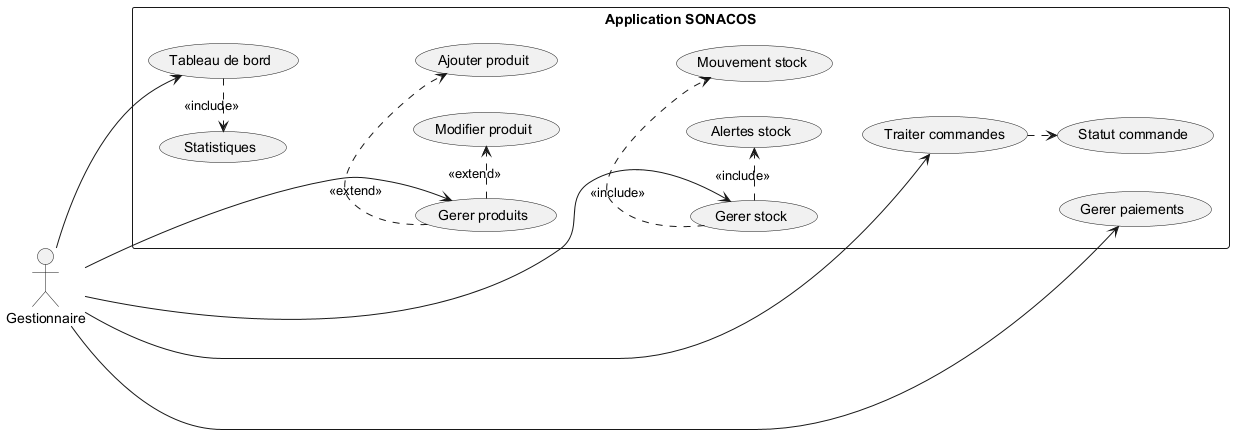
\includegraphics[width=0.92\textwidth,height=0.62\textheight,keepaspectratio]{usecase_gestionnaire.png}
  \caption{Diagramme PlantUML des cas d'utilisation du gestionnaire}
  \label{fig:uc-plantuml-gestionnaire}
\end{figure}

\paragraph{Objectif.}
Le gestionnaire pilote les opérations commerciales et logistiques : produits, stock, commandes, paiements et indicateurs utiles au suivi quotidien.

\paragraph{Preconditions.}
\begin{itemize}
  \item L'utilisateur doit etre authentifie avec le role \texttt{GESTIONNAIRE}.
  \item Les actions d'ajout ou de modification de produit doivent respecter les champs obligatoires : nom, reference, categorie, prix, conditionnement et stock.
  \item Les mouvements de stock doivent etre lies a un produit existant.
\end{itemize}

\paragraph{Scenario nominal de gestion produit.}
\begin{enumerate}
  \item Le gestionnaire ouvre l'espace produits.
  \item Le systeme affiche la liste paginee des produits avec recherche et filtres.
  \item Le gestionnaire ajoute une nouvelle reference ou modifie un produit existant.
  \item Il renseigne le nom, la reference, la categorie, le prix, le conditionnement, la description et l'image.
  \item Le systeme valide les champs et enregistre la modification.
  \item Le produit devient visible ou masque dans le catalogue selon son statut actif.
\end{enumerate}

\paragraph{Scenario nominal de gestion stock.}
\begin{enumerate}
  \item Le gestionnaire ouvre le module stock.
  \item Il choisit un produit et le type de mouvement : entree, sortie ou correction.
  \item Il renseigne la quantite et le motif.
  \item Le systeme met a jour le stock disponible.
  \item Le mouvement est historise pour permettre le contrôle ulterieur.
\end{enumerate}

\paragraph{Cas alternatifs.}
\begin{itemize}
  \item Si la reference produit existe deja, le systeme refuse l'enregistrement.
  \item Si une sortie de stock depasse la quantite disponible, le systeme bloque l'operation.
  \item Si une commande est deja finalisee, certaines modifications deviennent indisponibles.
\end{itemize}

\subsubsection{Responsable}

\begin{figure}[H]
  \centering
  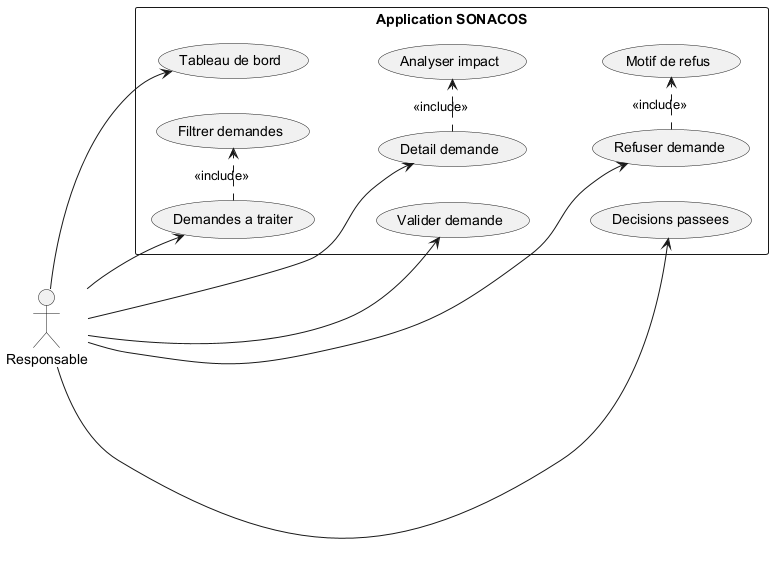
\includegraphics[width=0.92\textwidth,height=0.62\textheight,keepaspectratio]{usecase_responsable.png}
  \caption{Diagramme PlantUML des cas d'utilisation du responsable}
  \label{fig:uc-plantuml-responsable}
\end{figure}

\paragraph{Objectif.}
Le responsable contrôle les opérations necessitant une decision : validations sensibles, refus motives et consultation de l'historique des decisions.

\paragraph{Scenario nominal.}
\begin{enumerate}
  \item Le responsable ouvre son tableau de bord.
  \item Le systeme affiche le nombre de demandes en attente, les urgences et les decisions recentes.
  \item Le responsable filtre les demandes par type, priorite ou statut.
  \item Il ouvre le detail d'une demande.
  \item Le systeme presente l'objet concerne, le demandeur, l'impact commercial ou stock et les informations utiles.
  \item Le responsable valide la demande si elle est conforme.
  \item Le systeme met a jour le statut et trace la decision dans le journal.
\end{enumerate}

\paragraph{Cas de refus.}
\begin{enumerate}
  \item Le responsable clique sur refuser.
  \item Le systeme impose la saisie d'un motif.
  \item Le responsable renseigne le motif de refus.
  \item Le systeme enregistre la decision, le motif, la date et l'utilisateur responsable.
\end{enumerate}

\paragraph{Cas alternatifs.}
\begin{itemize}
  \item Si la demande a deja ete traitee par un autre responsable, elle n'est plus modifiable.
  \item Si le motif de refus est vide, le systeme bloque la decision.
  \item Si une erreur API se produit, le statut local n'est pas modifie.
\end{itemize}

\subsubsection{Administrateur}

\begin{figure}[H]
  \centering
  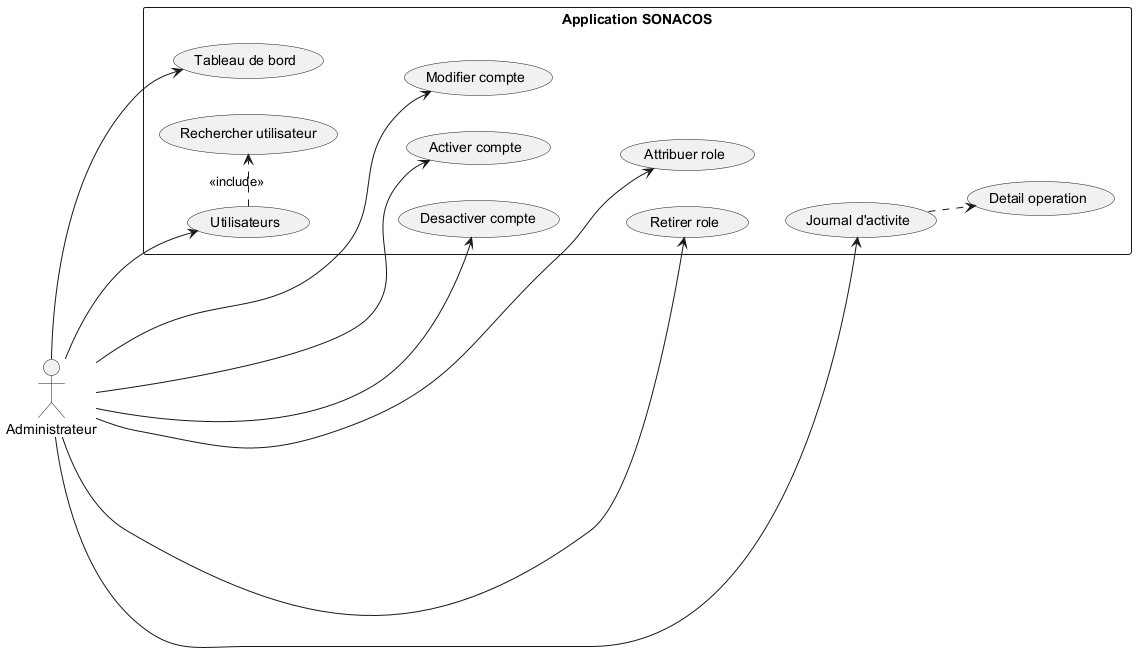
\includegraphics[width=0.92\textwidth,height=0.62\textheight,keepaspectratio]{usecase_admin.png}
  \caption{Diagramme PlantUML des cas d'utilisation de l'administrateur}
  \label{fig:uc-plantuml-admin}
\end{figure}

\paragraph{Objectif.}
L'administrateur gere la securite fonctionnelle de l'application : utilisateurs, activation des comptes, attribution des roles et consultation du journal d'activite.

\paragraph{Preconditions.}
\begin{itemize}
  \item L'utilisateur doit etre authentifie avec le role \texttt{ADMIN}.
  \item Les roles disponibles doivent exister dans le systeme.
  \item Les actions administratives doivent etre tracees.
\end{itemize}

\paragraph{Scenario nominal de modification utilisateur.}
\begin{enumerate}
  \item L'administrateur ouvre la page utilisateurs.
  \item Le systeme affiche la liste des comptes avec nom, email, ville, role, date de creation et statut.
  \item L'administrateur recherche un utilisateur.
  \item Il ouvre l'action modifier.
  \item Le systeme affiche les informations modifiables du compte.
  \item L'administrateur met a jour les champs autorises.
  \item Le systeme sauvegarde et affiche la nouvelle version du compte.
\end{enumerate}

\paragraph{Scenario nominal de gestion des roles.}
\begin{enumerate}
  \item L'administrateur selectionne un utilisateur.
  \item Il ajoute ou retire un role applicatif.
  \item Le systeme verifie que la modification est autorisee.
  \item Le systeme met a jour les droits d'acces.
  \item L'action est ajoutee au journal d'activite.
\end{enumerate}

\paragraph{Cas alternatifs.}
\begin{itemize}
  \item Si l'administrateur tente de retirer son propre role critique, le systeme doit empecher une perte d'acces.
  \item Si un compte est desactive, l'utilisateur concerne ne peut plus se connecter.
  \item Si une operation administrative echoue, le systeme conserve l'ancien etat.
\end{itemize}

\subsubsection{Archiviste}

\begin{figure}[H]
  \centering
  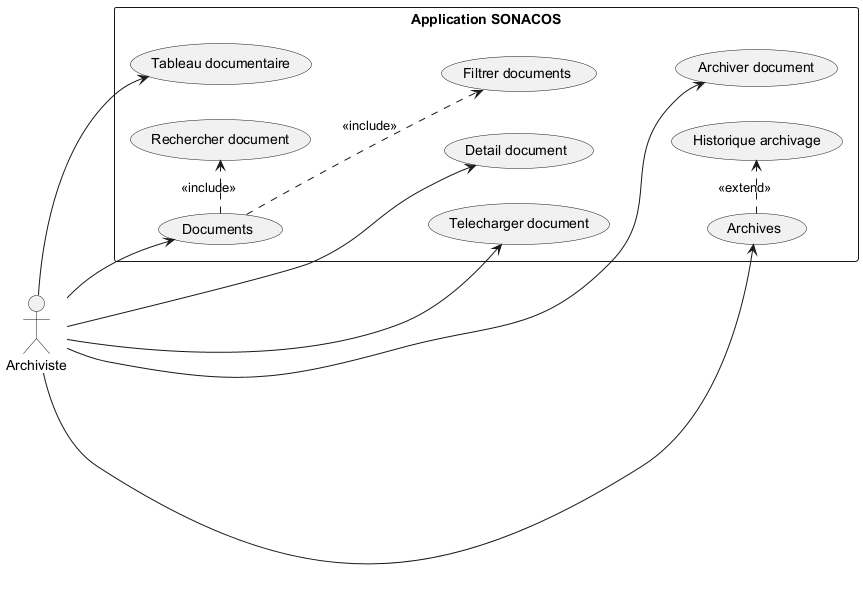
\includegraphics[width=0.92\textwidth,height=0.62\textheight,keepaspectratio]{usecase_archiviste.png}
  \caption{Diagramme PlantUML des cas d'utilisation de l'archiviste}
  \label{fig:uc-plantuml-archiviste}
\end{figure}

\paragraph{Objectif.}
L'archiviste centralise, consulte, telecharge et classe les documents commerciaux, principalement les factures et documents associes aux commandes.

\paragraph{Scenario nominal.}
\begin{enumerate}
  \item L'archiviste ouvre son tableau de bord documentaire.
  \item Le systeme affiche les documents disponibles, archives et en attente.
  \item L'archiviste filtre par type, statut ou date.
  \item Il ouvre le detail d'un document.
  \item Il telecharge le document pour vérification.
  \item Lorsque le document est conforme, il lance l'archivage.
  \item Le systeme marque le document comme archive et conserve l'historique.
\end{enumerate}

\paragraph{Cas alternatifs.}
\begin{itemize}
  \item Si le fichier PDF n'existe pas, le telechargement est bloque avec un message clair.
  \item Si le document est deja archive, le systeme evite un double archivage.
  \item Si l'utilisateur n'a pas le role archiviste, l'acces au module est refuse.
\end{itemize}

\subsubsection{Auditeur}

\begin{figure}[H]
  \centering
  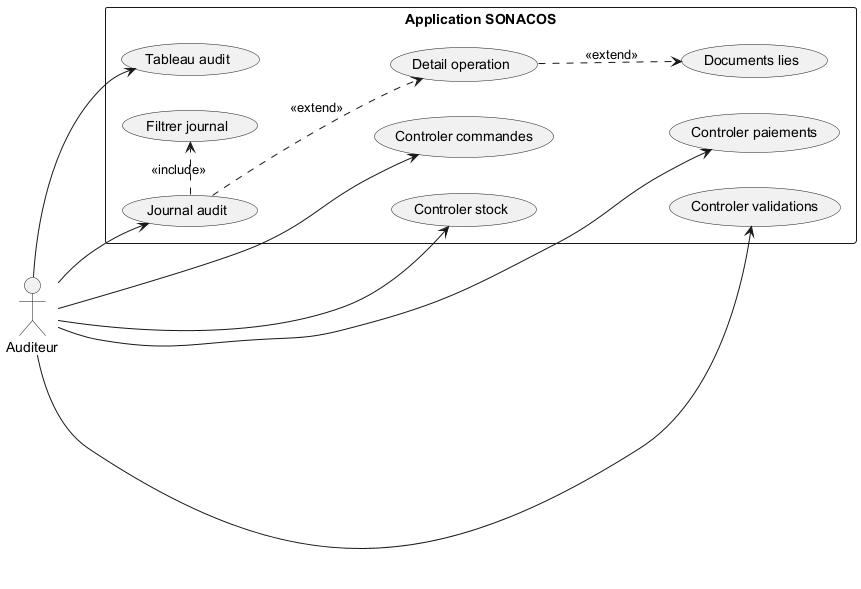
\includegraphics[width=0.92\textwidth,height=0.62\textheight,keepaspectratio]{usecase_auditeur.png}
  \caption{Diagramme PlantUML des cas d'utilisation de l'auditeur}
  \label{fig:uc-plantuml-auditeur}
\end{figure}

\paragraph{Objectif.}
L'auditeur contrôle les opérations sensibles en lecture seule. Il ne modifie pas les données, mais verifie la cohérence des commandes, paiements, stocks, validations et journaux.

\paragraph{Scenario nominal.}
\begin{enumerate}
  \item L'auditeur ouvre le tableau de bord audit.
  \item Le systeme affiche les indicateurs de contrôle et les opérations recentes.
  \item L'auditeur ouvre le journal d'audit.
  \item Il filtre par module, acteur, type d'action ou date.
  \item Il ouvre le detail d'une operation.
  \item Le systeme affiche l'utilisateur, l'action, l'objet concerne, la date et les informations associees.
  \item L'auditeur compare les informations avec les commandes, mouvements de stock, paiements ou validations.
\end{enumerate}

\paragraph{Cas alternatifs.}
\begin{itemize}
  \item Si aucune operation ne correspond aux filtres, un etat vide est affiche.
  \item Si l'operation n'existe plus, le systeme affiche une page d'information au lieu d'une erreur technique.
  \item Si l'auditeur tente une action de modification, le front-end et le back-end doivent la refuser.
\end{itemize}
